\documentclass[11pt]{article}
\usepackage{sectsty,graphicx,times,fancyhdr,cite,lastpage,url}
\allsectionsfont{\sffamily}
\pagestyle{fancy}
\fancyhf{}
\begin{document}
  \author{
    Danny Quist, Ph.D.\\
	Los Alamos National Laboratory\\
	Advanced Computing Solutions
  }
  \title{VERA Version 0.31\\User Manual and Documentation} 
  \maketitle
  \thispagestyle{empty} % Get rid of the page numbers on the first page
  \newpage
  \tableofcontents
  \newpage
\setcounter{page}{1}
%\rfoot{\thepage\ of \pageref{LastPage}}
\fancyhead[R]{\leftmark}
\fancyfoot[C]{Page \thepage\ of \pageref{LastPage}}

\section{Introduction}
VERA is a visualization tool for analyzing compiled executables. It is
built on an OpenGL framework with the wxWidgets package. The current
version is only for use with Windows XP and higher operating
systems. This manual will detail the steps that are needed to run and
analyze a sample of malware. 

There are two ways to generate trace data for VERA. The first is with
the Ether hypervisor. Ether is a set of patches made to the Xen hypervisor that
allows for covert analysis of running processes. It makes an ideal
environment to monitor and trace running programs. More information is
available from the Ether website.\footnote{Ether Website: \url{http://ether.gtisc.gtech.edu}} The next option is to use the VERAtrace Intel PIN module. This is a much simpler way of running traces and can be used inside any virtual machine. When available, choose the Ether system for generating traces. Ether is more resilient to detection over the Intel PIN-based VERAtrace.

\subsection{Recommended Hardware}

VERA is implemented using the OpenGL system with the wxWidgets API. In
order to get the best results out of VERA, we strongly recommend you
run it on a machine with a hardware graphics accelerator. The code was
developed using an Nvidia GTX 285 and subsequently tested on a variety
of other cards. 

\subsection{License and Copyright Information}

This program was prepared by Los Alamos National Security, LLC at Los
Alamos National Laboratory (LANL) under contract No. DE-AC52-06NA25396
with the U.S. Department of Energy (DOE). All rights in the program
are reserved by the DOE and Los Alamos National Security, LLC. The
U.S. Government retains ownership of all rights in the program and
copyright subsisting therein. All rights not granted below are
reserved. 

This program may be used for noncommercial, nonexclusive purposes for
internal research, development and evaluation and demonstration
purposes only. The right to reproduce, distribute, display publicly,
prepare derivative works or compilations thereof is prohibited.

NEITHER THE UNITED STATES NOR THE UNITED STATES DEPARTMENT OF ENERGY,
NOR THE LOS ALAMOS NATIONAL SECURITY, LLC, NOR ANY OF THEIR EMPLOYEES,
MAKES ANY WARRANTY, EXPRESS OR IMPLIED, OR ASSUMES ANY LEGAL LIABILITY
OR RESPONSIBILITY FOR THE ACCURACY, COMPLETENESS, OR USEFULNESS OF ANY
INFORMATION, APPARATUS, PRODUCT, OR PROCESS DISCLOSED, OR REPRESENTS
THAT ITS USE WOULD NOT INFRINGE PRIVATELY OWNED RIGHTS.

\section{Installing VERA}

Installing VERA is very straightforward. Simply download the package
from Offensive Computing\footnote{\url{http://www.offensivecomputing.net/vera/}} and
double-click on the installation file. The files will be installed
into the standard Program Files directory unless you specify
otherwise. 

To execute VERA either find the VERA directory in program files and
double-click the wxvera.exe file, or find the shortcut that was placed
in the Start menu or on the desktop. 

\section{Ether}

Installing the Ether patches to Xen can be an interesting
experience. This section will attempt to aide you in this process. As
always please consult with the official Georgia Tech Ether website for
the most up-to-date information.

\subsection{Installation Steps}

There are some general steps to install an Ether system. Most of the
problems that many people have are related to trying to compile the
source from scratch. To make this process easier we have provided a
precompiled Debian package. This alleviates many of the problems that
most are having with the installation. Following these steps exactly
will get you through much of the difficulty.

\begin{enumerate}
\item Download and install the Debian AMD64 net installation
ISO.\footnote{\url{http://www.debian.org/CD/netinst/}} You'll need to
get the ``Lenny'' release of Debian. Also make sure to get the 64-bit
version installed.
\item Install the required packages for a working Xen system. A
complete list can be found at Offensive Computing.\footnote{\url{http://www.offensivecomputing.net/ether_install_packages.log}}
\item Next install the Ether system. There are two methods for doing
this: from source or from a Debian package. We have prepared a Debian
package that may alleviate some of the problems of compiling from
source.\footnote{\url{http://www.offensivecomputing.net/?q=node/1575}}
\item Make sure that the Grub configuration matches your system
installation. While the package we have prepared does a decent job of
preparing the menu.lst file, there are some problems that may
arise. Figure~\ref{fig:menu_lst} has an example of a working
configuration file.
\item Reboot and verify that your new Xen/Ether system is up and
running.
\end{enumerate}

\begin{figure}[htb]
\centering
\begin{verbatim}
title Debian GNU/Linux, kernel 2.6.26-2-xen-amd64
root (hd0,0)
kernel /boot/xen-3.1.0.gz dom0_mem=1G
module /boot/vmlinuz-2.6.26-2-xen-amd64 root=/dev/sda1 ro quiet
module /boot/initrd.img-2.6.26-2-xen-amd64
\end{verbatim}
\caption{An example GRUB menu.lst file for a working Ether installation}\label{fig:menu_lst}
\end{figure}

\subsection{Setting up a Windows Virtual Machine}

Creating a virtual machine after Ether is installed can be
problematic. There is a bug that will freeze the installation during
the install program's execution. To get around this problem, simply
boot into a non-Ether patched system when you are first configuring a
VM.

Ensure that you have followed the VM installation instructions from
Georgia Tech.\footnote{\url{http://ether.gtisc.gatech.edu/xen_install_windows.pdf}}
Failure to create a proper VM will result in crashes and other
problems. Once your system is installed, you can begin taking traces for use
inside of VERA. 

\subsection{Generating Traces}

The primary unit of data that VERA operates on is a trace file. The
format for the traces is the output from the Ether
``instrtrace'' command. The output generally
contains a listing of addresses and the associated instruction that is
executed. VERA loads this trace file, processes it, then outputs a
graph markup language (GML) formatted file. VERA can display GML files
without any additional processing.

\subsection{Generating the Traces}
This section will overview generating traces inside of Ether. The
example that will be used is the notepad.exe file. First, start up a
virtual machine inside of the Ether system. Once the OS is booted,
the virtual machine ID will be needed. To find the ID, simply run the
``xm list'' command. This will display a listing of running virtual
machines. This ID is necessary to run Ether.

Next execute ether using the following command:

\begin{verbatim}ether_ctl instrace # notepad.exe > notepad.trace\end{verbatim}

Be sure to substitute the ``\#'' with the VM ID from the ``xm list''
command. This will generate a text listing of some initial Ether boilerplate,
and the instruction traces used to build the later GML file. Transfer
the notepad.trace file to the analysis machine where VERA is
installed. Section~\ref{sec:gui} details loading the trace files in
the GUI.

\subsection{Trace File Format}

If you would like to generate your own trace files for use in VERA,
they must have a specific format matching the Ether instruction
traces. The beginning of the file should match the output from
Figure~\ref{fig:boilerplate}. 

\begin{figure}[htb]
\centering
\begin{verbatim}
After init:
        shared_page_ptr: 0xffff830000fd9000
        shared_page_mfn: 0xfd9
        domid_source: 0
        event_channel_port: 34
Shared Page va: 0x7fde19b77000
Shared Page test:
        Page-Sharing is A-OK!

Trying to bind to local port...
Success, bound to local port: 35
Trying to get first pending notification...
Taking off suprious pending notification...
Setting filter by name to: notepad.exe
Execution of Target detected:
        Image Base:  0x1000000
        Image Size:  0x14000
        Entry Point: 0x100739d
\end{verbatim}
\caption{The starting boilerplate for an instruction trace.}\label{fig:boilerplate}
\end{figure}

Next will be the instruction traces. As
shown in Figure~\ref{fig:instructions}, the format is a hex virtual address,
that should match the contents of the executable, and the
ASCII representation of the instruction.  

\begin{figure}[htb]
\centering
\begin{verbatim}
100739d: push   0x70
100739d: push   0x70
100739f: push   0x01001898
10073a4: call   0x01007568
1007568: push   0x010075BA
100756d: mov    eax, fs:[0x00000000]
1007573: push   eax
\end{verbatim}
\caption{The contents of the instruction trace portion.}\label{fig:instructions}
\end{figure}

Finally, the end of the file should contain the string ``Handling
sigint'' twice. This denotes the end of a trace. Figure~\ref{fig:end}
shows an example of this data. Once this is
completed, the files should be parsable by VERA and will generate
graphs.

\begin{figure}[htb]
\centering
\begin{verbatim}
1007519: jnz	0x01007522
100751b: push	esi
100751c: call	[0x1001318]
Handling sigint
Handling sigint
\end{verbatim}
\caption{The ending structure of the trace file.}\label{fig:end}
\end{figure}

A full sample file can be found on the VERA webpage.\footnote{\url{http://www.offensivecomputing.net/vera/notepad.trace.gz}}

\section{Intel PIN-Based VERAtrace}\label{sec:pinvera}

VERAtrace is a tracing system based on the Intel PIN-monitoring
framework. It can be used to generate similar traces as can be found
from Ether, but does not require a full Xen/Ether installation. Traces
also include an import resolution system, which can be displayed in
the VERA GUI.

To generate traces, you will need the following files from the VERA
installation directory:

\begin{itemize}
\item pin.exe
\item pinvm.dll
\item taipin.dll
\item veratrace.dll
\end{itemize}

The above files may be copied to any virtual machine as long as it is
running in 32-bit mode. To run a trace, simply execute the command
listed in Figure~\ref{fig:veratrace}

\begin{figure}[htb]
\centering
\begin{verbatim}
pin.exe -t veratrace -- \\windows\\system32\\sol.exe
\end{verbatim}
\caption{Command line execution of veratrace of the Windows XP
Solitaire program}\label{fig:veratrace}
\end{figure}

The output will be a trace file with the name of the executable (minus
the directory) along with the PID used to run the program. The output
of the command in Figure~\ref{fig:veratrace} was the file named
``sol.exe-2015.trace''. This file can then be copied to the VERA directory and processed normally.

\section{VERA GUI and Usage}\label{sec:gui}

The VERA GUI is a front-end to allow you to quickly visualize and
explore a program's execution trace. After generating a trace file, VERA can be used to process and generate a graph. This
process converts the trace into a GML file that can be loaded and
explored in the GUI.

\subsection{Loading a Sample Trace File}

Included in the VERA executable distribution is a sample trace file
that contains a runtime trace of the ``notepad.exe'' program from a
standard Windows XP Service Pack 2 installation. To load the program,
simply use the open folder icon in the tool bar or the ``File/Open''
menus; find the trace file named ``notepad.trace''.


\begin{figure}[htb]
  \centering
  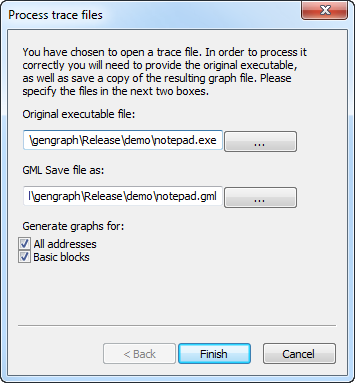
\includegraphics[width=3.5in]{vera-trace-dialog.png}
  \caption{The dialog for processing traces within VERA.}\label{vera:trace-gen}
\end{figure}


A separate window will open, resembling
Figure~\ref{vera:trace-gen}. Two pieces of information must be entered
in these fields. The first is the original executable for the
file. This file is needed to analyze the running sections of the
executable to color the graph. The second piece of information is the
name to use to store the GML file. The name you enter here will be the
source for the output names based on the type of graph you're looking
for. The next options are for processing a graph that has all the
addresses rendered as a node in the graph. Rendering all the addresses
as vertices is referred to as ``All Addresses'' mode. To only render the beginnings and ends of basic blocks, select the ``Basic Block'' check box. Once you are ready to process the trace file, click the ``Finish'' button. A new thread will be created to show you the results of the graph. Figure~\ref{vera:notepad-trace} shows the results of parsing the Notepad trace.

\begin{figure}[htb]
  \centering
  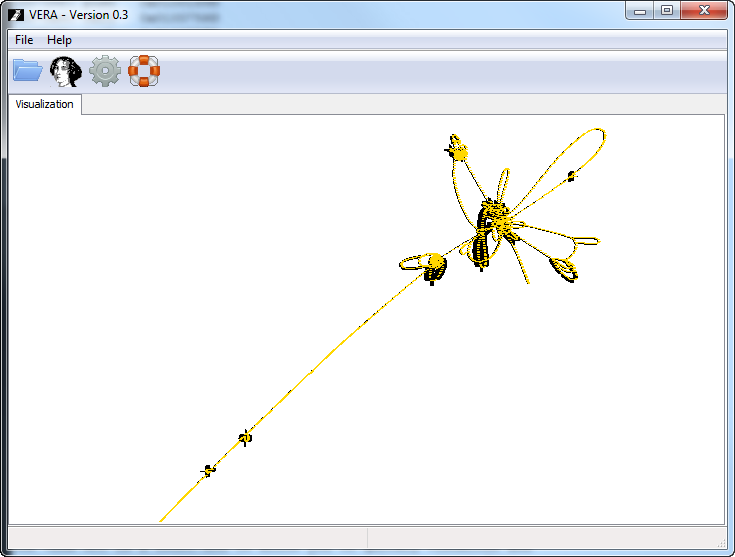
\includegraphics[width=4.0in]{vera-notepad-trace.png}
  \caption{The resulting graph from processing the Notepad trace.}\label{vera:notepad-trace}
\end{figure}

Depending on the options, two different graphs can be created. The
first will be the all vertices graph. This will have the name of
``all-yourgraphname.gml''. The second is the basic blocks graph. This will
have the name of ``bbl-yourgraphname.gml''. The default behavior is for
VERA to load the ``all-'' file. To load the basic blocks graph, load the ``bbl-'' file using the ``File/Open'' menus.


\subsection{Interacting with the Graph}

Interaction with the generated graphs was designed to emulate many
common 2D navigation systems. The interface is similar to that of Google Maps. There are two methods for moving a graph: First by panning left, right, up, and down. The second is to zoom in and out. All are accomplished with the mouse. Table~\ref{table:controls} lists each of the controls for interacting with the graph.

\begin{table}[htb]
\centering
\begin{tabular}{ | l | c | }
\hline
\bf{Action} & \bf{Mouse Control}\\
\hline
Pan Left & Left-click, drag left \\
Pan Right & Left-click, drag right \\
Zoom In & Mouse wheel up \\
Zoom Out & Mouse wheel down \\
Navigate in IDA & Right-click \\
\hline

\end{tabular}\caption{Mouse controls for navigation.}\label{table:controls}
\end{table}

\subsection{Identifiying Program Constructs in VERA}

Various features in the graph correlate to features inside of the
code. First, any series of addresses that have exactly one entrance
and one exit, and that are not part of a loop, can be safely
considered initialization code. Many of the constructs also show up in
multiple areas of the executable. The initialization portion of the
Notepad graph in Figure~\ref{vera:notepad-trace} shows an initial
series of instructions, followed by a loop prior to entering the main
portion of execution. This is a very common shape created by
Microsoft compilers. 

A section of code that shows a branching operation, such as
illustrated in Figure~\ref{fig:notepad-branch}, correlate to a decision
point in the program. Please note that if the branch always takes a
single path, the structure will not be shown in the graph. This is
because VERA relies upon traces of execution from the code, and does
not note the possible paths of execution available.

\begin{figure}[htb]
  \centering
  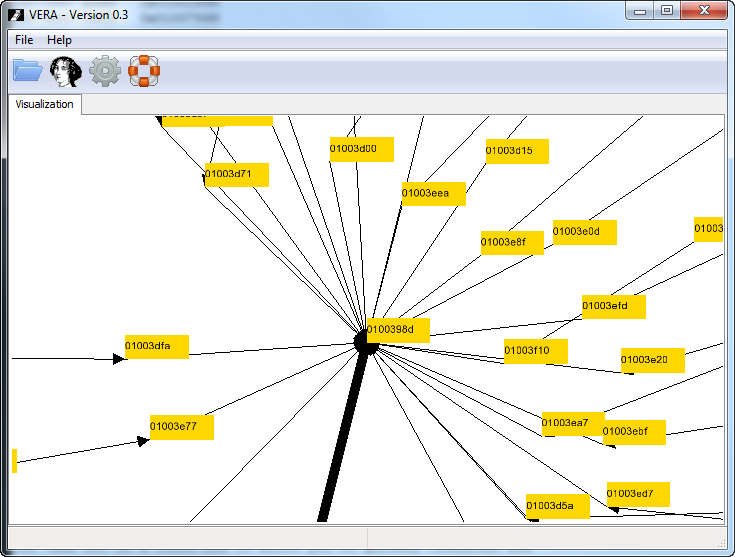
\includegraphics[width=5.0in]{vera-notepad-trace-zoom3.png}
  \caption{A series of branching operations from the Notepad.exe program.}\label{fig:notepad-branch}
\end{figure}

Whenever a portion of code is executed multiple times, the edges
between the nodes are drawn with a thicker width. This allows for
quicker identification of the most commonly used areas of code. For
instance, if a messaging processing loop is present in a program, that
loop will be highlighted. Figure~\ref{fig:notepad-loop} shows a loop
in the Notepad program.

\begin{figure}[htb]
  \centering
  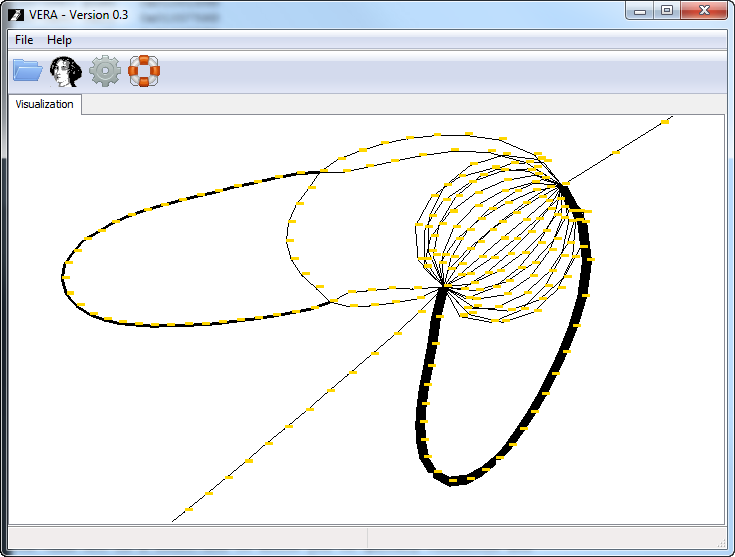
\includegraphics[width=5.0in]{vera-notepad-trace-zoom2.png}
  \caption{A loop with multiple branches inside the Notepad.exe program.}\label{fig:notepad-loop}
\end{figure}

\subsection{Interacting with IDA Pro}

A new feature in VERA 0.3 is the interaction capability with a program
loaded in IDA Pro. This alleviates the need to separately interact
with IDA and manually enter the addresses. To initiate a connection
to an IDA system, you will need a couple of things: First, of course,
is a copy of IDA Pro. The second is the VERA--IDA plugin for successful interaction with IDA. You can download a copy from
Offensive Computing.\footnote{\url{http://www.offensivecomputing.net/vera}}

Precompiled versions of the IDA module are available for IDA Pro versions 5.6 and later. The source code is available for earlier
versions of IDA, and you're welcome to try to compile it. They are
not, however, officially supported.

\begin{figure}[htb]
  \centering
  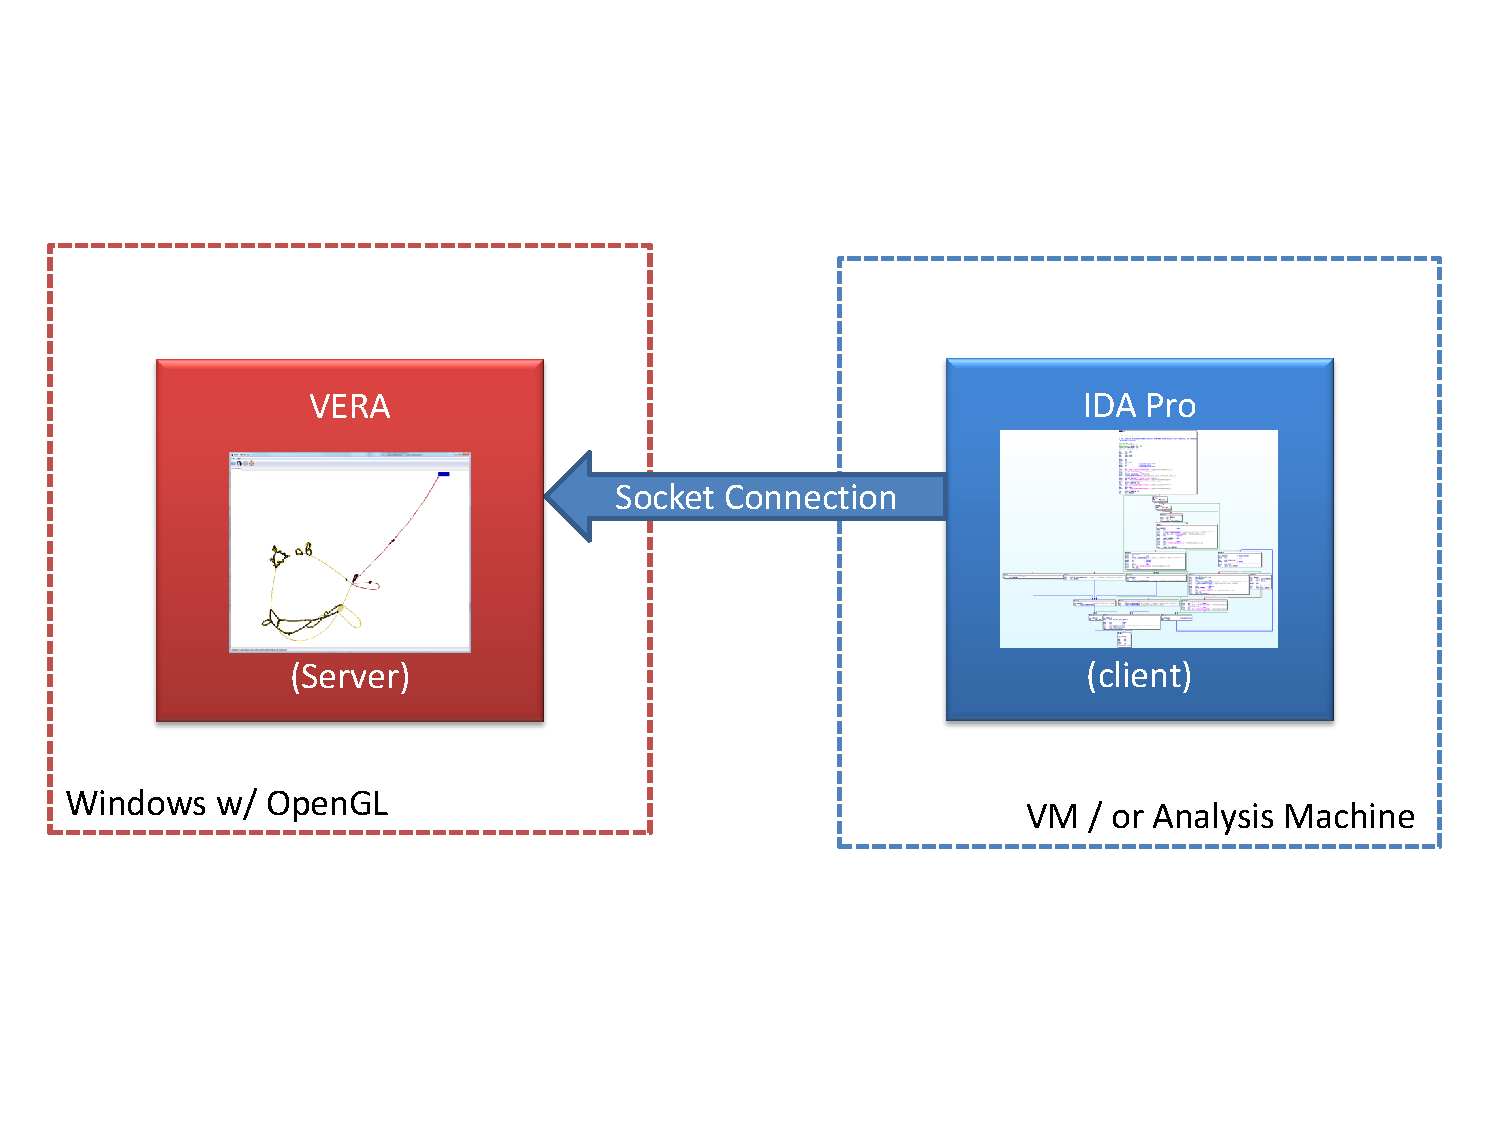
\includegraphics[width=5.0in]{architecture.pdf}
  \caption{Architecture of the VERA IDA Plugin}\label{fig:vera-ida-arch}
\end{figure}

The plugin should be copied into the ``plugins'' directory of the
IDA Pro installation directory. Once this has been done, you will need
to restart IDA.   

Once the module has been installed and IDA has been restarted, you
should see a message in your IDA console that looks very similar to
Figure~\ref{fig:vera_plugin}. If you do not see the message, then you
will need to verify that the IDA plugin was installed correctly. 

\begin{figure}[htb]
  \centering
  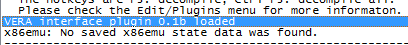
\includegraphics{vera-ida-text.png}
  \caption{IDA console text showing the IDA Pro module loaded correctly.}\label{fig:vera_plugin}
\end{figure}

To start the IDA Pro server, click on the IDA Pro icon in the VERA toolbar. From here the server should be started. Next, you will need to figure out the computer's IP address. A TCP/IP connection is made from the IDA Pro system to the VERA system. This allows you to take advantage of virtual machines when analyzing malware. This architecture was chosen to allow for an IDA Pro instance on a virtual machine talk to VERA running on a machine with a real hardware graphics accelerator. 


\newpage
%\bibliography{dissertation}{}
%\bibliographystyle{plain}

\end{document}
